\begin{enumerate}[label=\thesubsection.\arabic*,ref=\thesubsection.\theenumi]
\item  For station X, the maximum one day rainfall with 25 years return period is 100 mm.
The probability of a one day rainfall equal to or greater than 100 mm at station X occurring at least once in 15 successive years is
\hfill(AG 2007)
\begin{multicols}{4}
\begin{enumerate}
  \item 0.458
  \item 0.500
  \item 0.637
  \item 0.990
\end{enumerate}
\end{multicols}
\item If the standard deviation of the spot speed of vehicles in a highway is $8.8 kmph$ and the mean speed of the vehicles is $33 kmph$, the coefficient of variation in speed is
\hfill{\brak{\text{CE 2007}}}
\begin{multicols}{4}
\begin{enumerate}
\item 0.1517
\item 0.1867
\item 0.2666
\item 0.3646
\end{enumerate}
\end{multicols}
\item Suppose we uniformly and randomly select a permutation from the $20!$ permutations of $1,2,3,...,20.$ What is the probability that $2$ appears at an earlier position than any other even number  in selected permutation ?
\hfill {(CS 2007)}
\begin{enumerate}
    \begin{multicols}{4}
    \item $\frac{1}{2}$   

    \item $\frac{1}{10}$

    \item $\frac{9!}{20!}$
  
    \item None of these
    \end{multicols}
\end{enumerate}
    \item There are $n$ stations in a slotted LAN. Each station attempts to transmit with a probability $p$ in each time slot. What is the probability that {ONLY} one station transmits in a given time slot?  
\hfill {(CS 2007)}
    \begin{enumerate}
    \begin{multicols}{4}
        \item $np(1-p)^{n-1}$
        \item $(1-p)^{n-1}$
        \item $p(1-p)^{n-1}$
        \item $1 - (1-p)^{n-1}$
        \end{multicols}
    \end{enumerate}

\item If $ E $ denotes expectation, the variance of a random variable $ X $ is given by:
\hfill{\brak{\text{EC 2007}}}
    \begin{multicols}{2}
\begin{enumerate}
    \item $ E[X^2] - E^2[X] $
    \item $ E[X^2] + E^2[X] $
    \item $ E[X^2] $
    \item $ E^2[X] $
\end{enumerate}
\end{multicols}
\item If $ R(\tau) $ is autocorrelation of real, WSS random process, which is NOT true: 
\hfill{\brak{\text{EC 2007}}}
\begin{enumerate}
    \item $ R(\tau) = R(-\tau) $
    \item $ |R(t)| \leq R(0) $
    \item $ R(\tau) = -R(-\tau) $
    \item Mean square value is $ R(0) $
\end{enumerate}

\item If $ S(f) $ is power spectral density of a real WSS random process, which is ALWAYS true: 

\hfill{\brak{\text{EC 2007}}}
\begin{multicols}{4}
\begin{enumerate}
    \item $ S(0) \geq S(f) $
    \item $ S(f) \geq 0 $
    \item $ S(-f) = -S(f) $
    \item $ \int S(f) df = 0 $
\end{enumerate}
\end{multicols}
\item An examination consists of two papers, Paper I and Paper II. The probability of failing in Paper I is 0.3 and that in Paper II is 0.2. Given that a student has failed in Paper II, the probability of failing in Paper I is 0.6. The probability of a student failing in both the papers is: 
\hfill{\brak{\text{EC 2007}}}
\begin{multicols}{4}
\begin{enumerate}
    \item 0.5
    \item 0.18
    \item 0.12
    \item 0.06
\end{enumerate}
\end{multicols}
\item During transmission over a binary channel, bit errors occur independently with probability $p$. The probability of {at most one} bit in error in a block of $n$ bits is: 
\hfill{\brak{\text{EC 2007}}}
\begin{multicols}{2}
    

\begin{enumerate}
    \item $p^n$
    \item $1-p^n$
    \item $np(1-p)^{n-1} + (1-p)^n$
    \item $1-(1-p)^n$
\end{enumerate}
\end{multicols}

\item  Two 4-ary signal constellations are shown. It is given that $\phi_1$ and $\phi_2$ constitute an orthonormal basis and four symbols in each are equiprobable. Let $N_0/2$ denote the power spectral density of white Gaussian noise. 
\hfill{\brak{\text{EC 2007}}}

\begin{figure}[H]
    \centering
    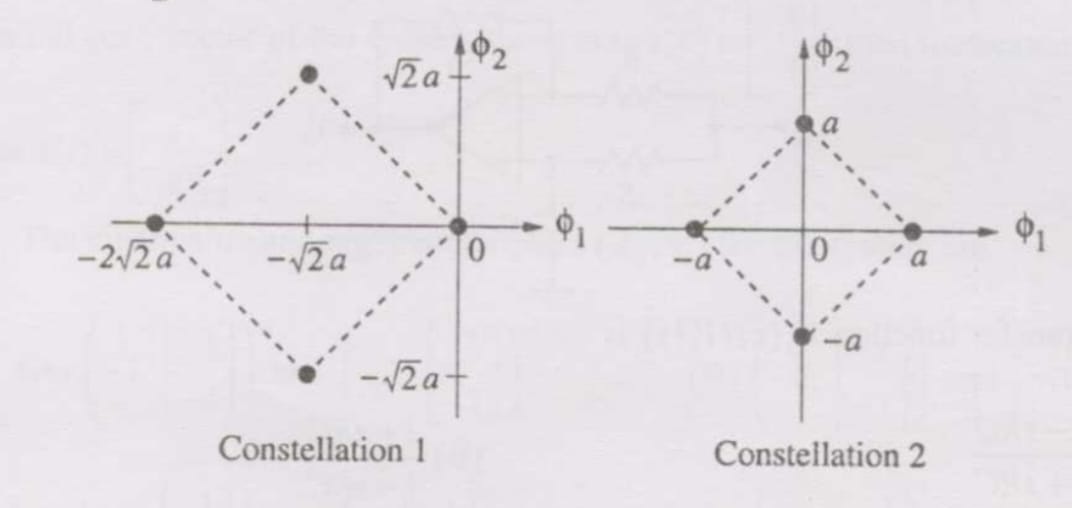
\includegraphics[width=0.6\textwidth]{figs/2007/EC/Q74Q75.jpg}
    \caption{}
    \label{fig:Q74@75.jpg}
\end{figure}

\begin{enumerate}
\item The ratio of the average energy of Constellation 1 to that of Constellation 2 is:
\begin{multicols}{4}
\begin{enumerate}
  \item $4a^2$
  \item $4$
  \item $2$
  \item $8$
\end{enumerate}
\end{multicols}


\item If these constellations are used over an AWGN channel, then:
\begin{enumerate}
  \item Probability of symbol error for Constellation 1 is lower
  \item Probability of symbol error for Constellation 1 is higher
  \item Probability of symbol error is equal for both
  \item Value of $N_0$ will determine which has lower error
\end{enumerate}
\end{enumerate}

\item
An input to a 6-level quantizer has PDF $f(x)$ as shown: it is piecewise-constant with three decision boundaries at $-1$, $0$, and $1$, chosen to maximize output entropy. The central plateau height is $a$, the outer flat region height is $b$. 
\hfill{\brak{\text{EC 2007}}}
\begin{figure}[H]
    \centering
    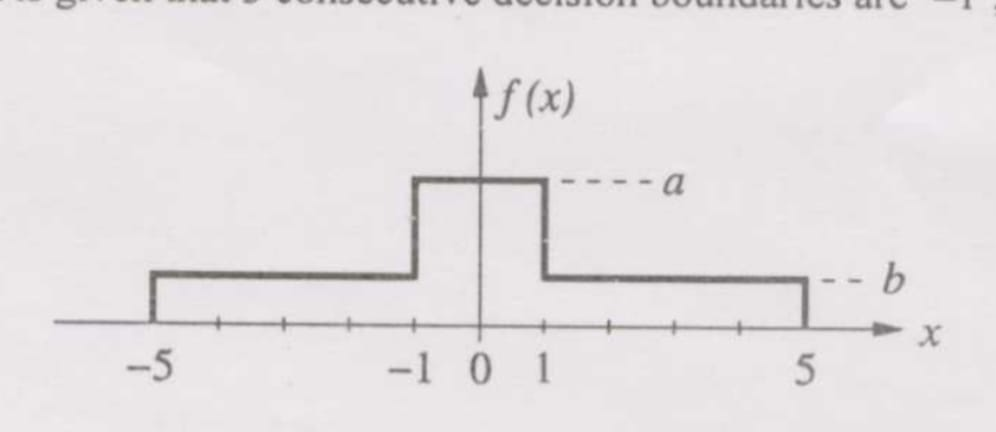
\includegraphics[width=0.4\textwidth]{figs/2007/EC/Q82Q83.jpg}
    \caption{}
    \label{fig:Q82Q83.jpg}
\end{figure}

\begin{enumerate}
\item The values of $a$ and $b$ are:
\begin{multicols}{4}
\begin{enumerate}
  \item $a=\tfrac{1}{6},\ b=\tfrac{1}{12}$
  \item $a=\tfrac{1}{5},\ b=\tfrac{3}{40}$
  \item $a=\tfrac{1}{4},\ b=\tfrac{1}{16}$
  \item $a=\tfrac{1}{3},\ b=\tfrac{1}{24}$
\end{enumerate}
\end{multicols}

\item Assuming reconstruction levels are midpoints of decision intervals, the ratio of signal power to quantization noise power is:

\begin{multicols}{4}
\begin{enumerate}
  \item $\frac{152}{9}$
  \item $\frac{64}{3}$
  \item $\frac{76}{3}$
  \item $28$
\end{enumerate}
\end{multicols}
\end{enumerate}

\item  A loaded dice has following probability distribution of occurrences
%
\begin{center}
\begin{tabular}{|c|c|c|c|c|c|c|}
\hline
Dice value      & 1   & 2   & 3   & 4   & 5   & 6   \\
\hline
Probability     & $1/4$ & $1/8$ & $1/8$ & $1/8$ & $1/8$ & $1/4$ \\
\hline
\end{tabular}
\end{center}
%
If three identical dice as the above are thrown, the probability of occurrence of values 1, 5 and 6 on the three dice is\hfill{(EE 2007)} 
% 
\begin{enumerate}
    \item same as that of occurrence of 3, 4, 5
    \item same as that of occurrence of 1, 2, 5
    \item$1/128$
    \item $5/8$
\end{enumerate}
%
\item A coin is tossed thrice. Let X be the event that head occurs in each of the first two tosses.  
Let Y be the event that a tail occurs on the third toss.  
Let Z be the event that two tails occur in three tosses.  
Based on the above information, which one of the following statements is TRUE?  
\hfill (GE 2007)
\begin{multicols}{2}
\begin{enumerate}
\item X and Y are not independent  
\item Y and Z are dependent  
\item Y and Z are independent  
\item X and Z are independent  
\end{enumerate}
\end{multicols}
\item Assume that the duration in minutes of a telephone conversation follows the exponential distribution $$f(x) = \frac{1}{5} e^{-x/5}, x \geq 0$$. The probability that the conversation will exceed five minutes is  
\hfill(IN 2007)
\begin{multicols}{4}
\begin{enumerate}
\item $\frac{1}{e}$  
\item $\frac{1}{5}$  
\item $\frac{1}{3}$  
\item $1 - \frac{1}{e}$  
\end{enumerate}
\end{multicols}
\item Two sensors have measurement errors that are Gaussian distributed with zero means and variances $\sigma_1^2$ and $\sigma_2^2$, respectively. The two sensor measurements $x_1$ and $x_2$ are combined to form the weighted average $x = \alpha x_1 + (1-\alpha)x_2, \, 0 \leq \alpha \leq 1$. Assuming that the measurement errors of the two sensors are uncorrelated, the weighting factor $\alpha$ that yields the smallest error variance of $x$ is  
\hfill(IN 2007)
\begin{multicols}{4}
\begin{enumerate}
\item $\frac{\sigma_1^2}{\sigma_1^2 + \sigma_2^2}$  
\item $\frac{\sigma_2^2}{\sigma_1^2 + \sigma_2^2}$  
\item $\frac{\sigma_1}{\sigma_1 + \sigma_2}$  
\item 0.5  
\end{enumerate}
\end{multicols}

\item The value of the integral $\int_{0}^{\infty} \int_{0}^{\infty} e^{-x^2-y^2} \, dx\, dy$ is  
\hfill(IN 2007)
\begin{multicols}{4}
\begin{enumerate}
\item $\sqrt{\pi}/2$  
\item $\sqrt{\pi}$  
\item $\pi$  
\item $\pi/4$  
\end{enumerate}
\end{multicols}

\end{enumerate}

